%!TEX root = ../Chapter3.tex
\begin{figure*}[t!]
\centering
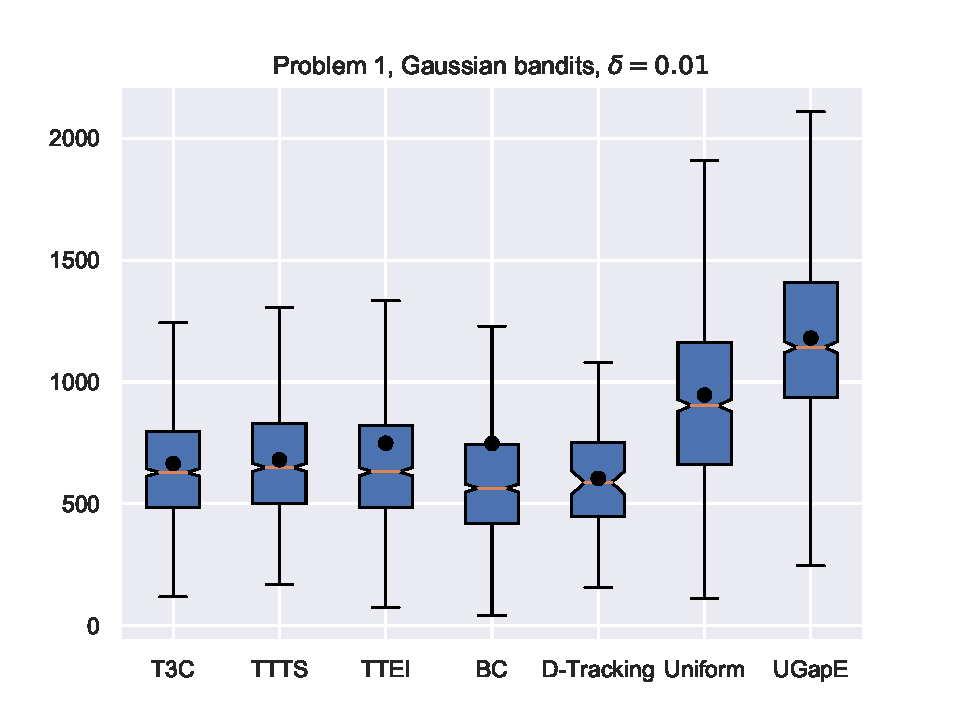
\includegraphics[clip, width= 0.24\textwidth]{Chapter3/img/gaussian1.pdf}
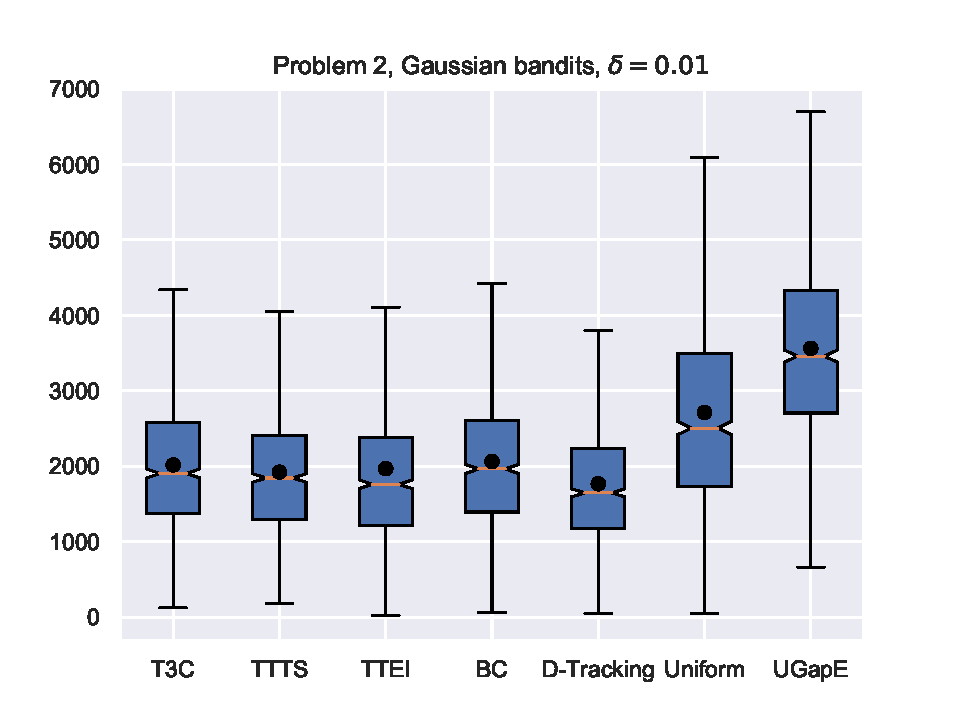
\includegraphics[clip, width= 0.24\textwidth]{Chapter3/img/gaussian2.pdf}
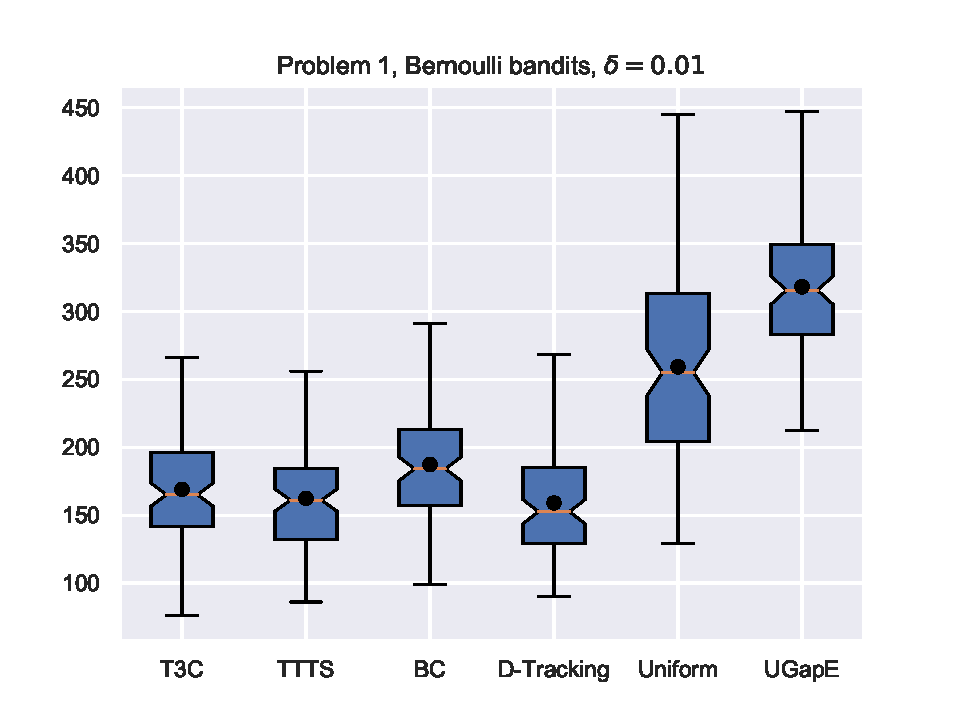
\includegraphics[clip, width= 0.24\textwidth]{Chapter3/img/bernoulli1.pdf}
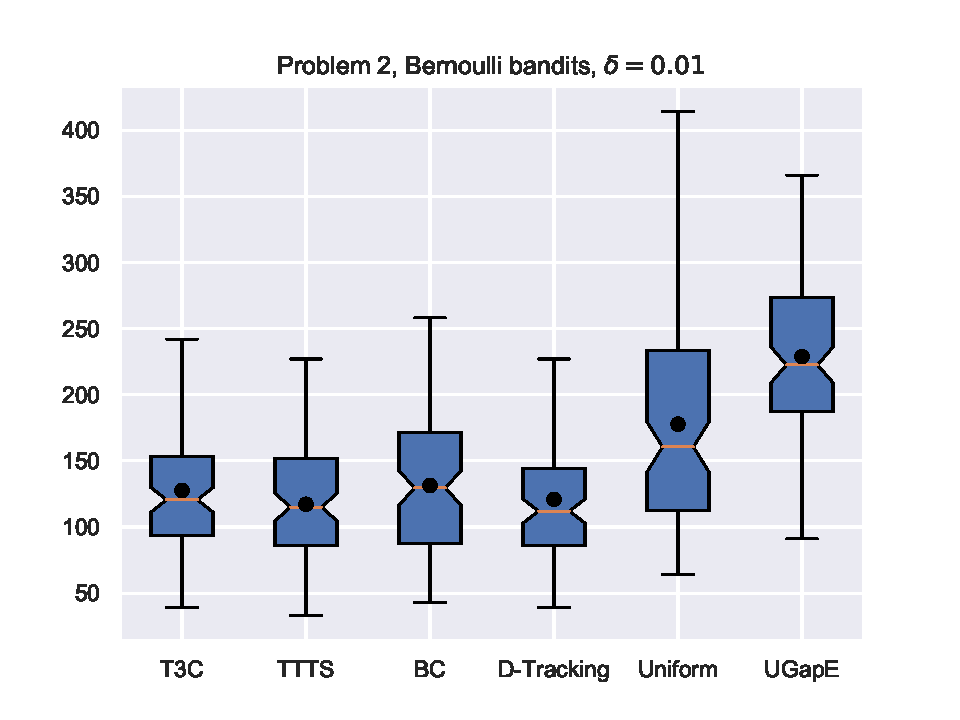
\includegraphics[clip, width= 0.24\textwidth]{Chapter3/img/bernoulli2.pdf}
\caption{Sample complexity of different BAI sampling rules over some random problem instances. Black dots represent means and oranges lines represent medians.}
\label{fig:confidence}
\end{figure*}

\begin{table*}[t!]
\centering
\small
%\def\arraystretch{1.2}
\begin{tabular}{|c|c|c|c|c|c|c|c|}
 \hline
 \textbf{Sampling rule} & \TCC & \TTTS & \TTEI & \BC & \DT & \texttt{Uniform} & \UGapE \\
 \hline
 \textbf{Execution time (s)} & $1.6\times 10^{-5}$ & $2.3\times 10^{-4}$ & $1\times 10^{-5}$ & $1.4\times 10^{-5}$ & $1.3\times 10^{-3}$ & $6\times 10^{-6}$ & $5\times 10^{-6}$ \\
 \hline
\end{tabular}
\caption{Average execution time in seconds for different BAI sampling rules.}
\label{table:time}
\end{table*}


\section{Optimal Posterior Convergence
}\label{sec:bayesian}

Recall that $a_{n, I^\star}$ denotes the posterior mass assigned to the event that action $I^\star$ (i.e.\ the true optimal arm) is optimal at time $n$. As the number of observations tends to infinity, we desire that the posterior distribution converges to the truth. In this section we show equivalently that the posterior mass on the complementory event, $1 - a_{n, I^\star}$, the event that arm $I^\star$ is not optimal, converges to zero at an exponential rate, and that it does so at optimal rate $\Gamma_{\beta}^\star$. 

\citet{russo2016ttts} proves a similar theorem under three confining boundedness assumptions (cf.\,\citealt{russo2016ttts}, Asssumption 1) on the parameter space, the prior density and the (first derivative of the) log-normalizer of the exponential family. Hence, the theorems in \cite{russo2016ttts} do not apply to the two bandit models most used in practise, which we consider in this paper: the Gaussian and Bernoulli model. 

In the first case, the parameter space is unbounded, in the latter model, the derivative of the log-normalizer (which is $e^{\eta} / (1 + e^\eta)$) is unbounded. Here we provide two theorems, proving that under \TTTS, the optimal, exponential posterior convergence rates are obtained for the Gaussian model with uninformative (improper) Gaussian priors (proof given in Appendix~\ref{app:posterior_gaussian}), and the Bernoulli model with $\cB eta(1,1)$ priors (proof given in Appendix~\ref{app:posterior_beta}).

\begin{restatable}{theorem}{restateposteriorgaussian}\label{thm:posterior_gaussian}
    Under \TTTS, for Gaussian bandits with improper Gaussian priors, it holds almost surely that 
    \[
        \lim_{n\rightarrow{\infty}} -\frac{1}{n}\log(1-a_{n,I^\star}) = \Gamma_{\beta}^\star.
    \]
\end{restatable}

\begin{restatable}{theorem}{restateposteriorbernoulli}\label{thm:posterior_bernoulli}
	Under \TTTS, for Bernoulli bandits and uniform priors, it holds almost surely that
	\[
	\lim_{n\rightarrow{\infty}} -\frac{1}{n}\log(1-a_{n,I^\star}) = \Gamma_{\beta}^\star.
	\]
\end{restatable}
